% smooth numbers up to 1e7 with Rankin bound (generated by a script).
\begin{tikzpicture}[x=1cm,y=1cm]
\draw[black!35] (0,0) rectangle (8.00,4.00);
\draw[black!35] (0.00,0)--(0.00,-0.08) node[below,font=\tiny,black!60]{$1$};
\draw[black!35] (2.00,0)--(2.00,-0.08) node[below,font=\tiny,black!60]{$10$};
\draw[black!35] (4.00,0)--(4.00,-0.08) node[below,font=\tiny,black!60]{$10^2$};
\draw[black!35] (6.00,0)--(6.00,-0.08) node[below,font=\tiny,black!60]{$10^3$};
\draw[black!35] (8.00,0)--(8.00,-0.08) node[below,font=\tiny,black!60]{$10^4$};
\draw[black!35] (0,0.00)--(-0.08,0.00) node[left,font=\tiny,black!60]{$0$};
\draw[black!35] (0,1.00)--(-0.08,1.00) node[left,font=\tiny,black!60]{$2$};
\draw[black!35] (0,2.00)--(-0.08,2.00) node[left,font=\tiny,black!60]{$4$};
\draw[black!35] (0,3.00)--(-0.08,3.00) node[left,font=\tiny,black!60]{$6$};
\draw[black!35] (0,4.00)--(-0.08,4.00) node[left,font=\tiny,black!60]{$8$};
\node[below,font=\tiny,black!60] at (4.00,-0.35) {$y$ (logarithmic scale)};
\node[rotate=90,font=\tiny,black!60] at (-0.75,2.00) {$\log_{10}$};
\draw[red!70!black,thick] (0.602,0.905) -- (0.954,1.423) -- (1.204,1.423) -- (1.556,1.767) -- (1.690,2.020) -- (2.000,2.020) -- (2.228,2.354) -- (2.511,2.473) -- (2.760,2.661) -- (3.010,2.794) -- (3.246,2.896) -- (3.496,3.016) -- (3.750,3.153) -- (4.000,3.233) -- (4.248,3.334) -- (4.501,3.415) -- (4.749,3.493) -- (4.999,3.562) -- (5.251,3.620) -- (5.499,3.670) -- (5.750,3.722) -- (6.000,3.766) -- (6.250,3.807) -- (6.500,3.842) -- (6.750,3.874) -- (7.000,3.903) -- (7.250,3.931) -- (7.500,3.956) -- (7.750,3.978) -- (8.000,4.000);
\draw[blue!70!black,thick] (0.602,0.690) -- (0.954,1.139) -- (1.204,1.139) -- (1.556,1.443) -- (1.690,1.667) -- (2.000,1.667) -- (2.228,1.959) -- (2.511,2.063) -- (2.760,2.227) -- (3.010,2.342) -- (3.246,2.430) -- (3.496,2.532) -- (3.750,2.649) -- (4.000,2.716) -- (4.248,2.801) -- (4.501,2.867) -- (4.749,2.932) -- (4.999,2.989) -- (5.251,3.037) -- (5.499,3.077) -- (5.750,3.119) -- (6.000,3.154) -- (6.250,3.187) -- (6.500,3.215) -- (6.750,3.240) -- (7.000,3.263) -- (7.250,3.285) -- (7.500,3.304) -- (7.750,3.321) -- (8.000,3.336);
\fill[blue!70!black] (0.602,0.690) circle (0.03cm);
\fill[blue!70!black] (0.954,1.139) circle (0.03cm);
\fill[blue!70!black] (1.204,1.139) circle (0.03cm);
\fill[blue!70!black] (1.556,1.443) circle (0.03cm);
\fill[blue!70!black] (1.690,1.667) circle (0.03cm);
\fill[blue!70!black] (2.000,1.667) circle (0.03cm);
\fill[blue!70!black] (2.228,1.959) circle (0.03cm);
\fill[blue!70!black] (2.511,2.063) circle (0.03cm);
\fill[blue!70!black] (2.760,2.227) circle (0.03cm);
\fill[blue!70!black] (3.010,2.342) circle (0.03cm);
\fill[blue!70!black] (3.246,2.430) circle (0.03cm);
\fill[blue!70!black] (3.496,2.532) circle (0.03cm);
\fill[blue!70!black] (3.750,2.649) circle (0.03cm);
\fill[blue!70!black] (4.000,2.716) circle (0.03cm);
\fill[blue!70!black] (4.248,2.801) circle (0.03cm);
\fill[blue!70!black] (4.501,2.867) circle (0.03cm);
\fill[blue!70!black] (4.749,2.932) circle (0.03cm);
\fill[blue!70!black] (4.999,2.989) circle (0.03cm);
\fill[blue!70!black] (5.251,3.037) circle (0.03cm);
\fill[blue!70!black] (5.499,3.077) circle (0.03cm);
\fill[blue!70!black] (5.750,3.119) circle (0.03cm);
\fill[blue!70!black] (6.000,3.154) circle (0.03cm);
\fill[blue!70!black] (6.250,3.187) circle (0.03cm);
\fill[blue!70!black] (6.500,3.215) circle (0.03cm);
\fill[blue!70!black] (6.750,3.240) circle (0.03cm);
\fill[blue!70!black] (7.000,3.263) circle (0.03cm);
\fill[blue!70!black] (7.250,3.285) circle (0.03cm);
\fill[blue!70!black] (7.500,3.304) circle (0.03cm);
\fill[blue!70!black] (7.750,3.321) circle (0.03cm);
\fill[blue!70!black] (8.000,3.336) circle (0.03cm);
\draw[black!60,densely dashed] (1.690,0.000) -- (2.000,0.474) -- (2.228,0.962) -- (2.511,1.421) -- (2.760,1.734) -- (3.010,1.983) -- (3.246,2.176) -- (3.496,2.345) -- (3.750,2.488) -- (4.000,2.606) -- (4.248,2.706) -- (4.501,2.793) -- (4.749,2.868) -- (4.999,2.933) -- (5.251,2.991) -- (5.499,3.040) -- (5.750,3.084) -- (6.000,3.123) -- (6.250,3.157) -- (6.500,3.189) -- (6.750,3.218) -- (7.000,3.244) -- (7.250,3.267) -- (7.500,3.288) -- (7.750,3.306) -- (8.000,3.322);
\draw[green!50!black,thick] (2.228,0.000) -- (2.511,0.661) -- (2.760,1.050) -- (3.010,1.259) -- (3.246,1.427) -- (3.496,1.630) -- (3.750,1.562) -- (4.000,1.681) -- (4.248,1.848) -- (4.501,1.997) -- (4.749,1.553) -- (4.999,1.659) -- (5.251,1.761) -- (5.499,1.856) -- (5.750,1.968) -- (6.000,2.073) -- (6.250,2.185) -- (6.500,2.288) -- (6.750,2.394) -- (7.000,2.498) -- (7.250,1.381) -- (7.500,1.434) -- (7.750,1.489) -- (8.000,1.545);
\draw[red!70!black,thick] (0.15,3.80)--(0.55,3.80) node[right,font=\tiny,black]{Rankin's bound, best $\sigma$};
\draw[blue!70!black,thick] (0.15,3.50)--(0.55,3.50) node[right,font=\tiny,black]{$\Psi(10^7,y)$};
\draw[black!60,densely dashed] (0.15,3.20)--(0.55,3.20) node[right,font=\tiny,black]{$10^7\rho(u)$};
\draw[green!50!black,thick] (0.15,2.90)--(0.55,2.90) node[right,font=\tiny,black]{$\binom{\pi(y)}{\lfloor u\rfloor}$};
\end{tikzpicture}
